\documentclass[../main.tex]{subfiles}

\begin{document}

\section{Higgs boson}%
\label{sec:higgs_boson}

\subsection{De nood voor een scalair boson}%
\label{sub:de_noot_voor_een_scalair_boson}

Bekijken we de cross secties van een aantal zelf interacties die kunnen plaatsvinden voor de zwakke interactie bosonen dan zien we bij ongeveer 1TeV dat de unitariteit geschonden wordt, de waarschijnlijkheden voor deze diagrammen worden groter dan 1.

\begin{figure}[h]
    \centering
    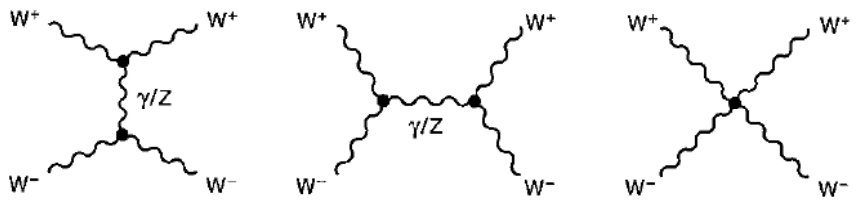
\includegraphics[width=0.8\linewidth]{higgs_boson/zwak_zelf_int_geen_H.png}
    \caption{Mogelijke zelf interactie diagrammen voor het toevoegen van Higgs interacties}%
    \label{fig:higgs_boson/zwak_zelf_int_geen_H}
\end{figure}

Om deze divergenties op te lossen is het nodig om extra parameters toe te voegen. Door het toevoegen van de de koppeling van de $W$ bosonen aan het Higgs boson, een scalair boson, is het mogelijk om de divergentie naar oneindig te convergeren.

\begin{figure}[h]
    \centering
    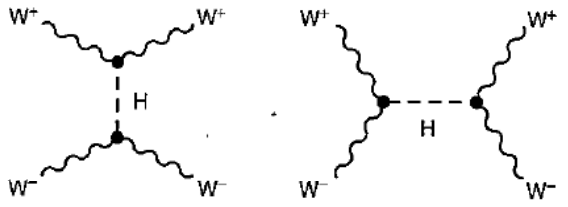
\includegraphics[width=0.6\linewidth]{higgs_boson/zwak_zelf_int_H.png}
    \caption{Toevoegen van Higgs boson interacties}%
    \label{fig:higgs_boson/zwak_zelf_int_H}
\end{figure}

We kunnen aan deze diagrammen direct zien dat de elektrozwakke koppeling van $W$ aan $Z$ een grote invloed zal hebben voor de koppeling van $W$ aan $H$. De opheffing van de divergenties zal enkel werken als de $H$-koppeling gerelateerd is aan de elektrozwakke koppeling.

\subsection{Lagrangiaan}%
\label{sub:lagrangiaan}

Hier moeten we overstappen van het relativistische beeld naar de kwantumvelden theorie omdat Higgs mechanisme en het bestaan van het Higgs boson niet uitgelegd kan worden zonder deze theorie.\\
Klassiek gezien is de Lagrangiaan niets meer dan $L(q_i, \dot{q}_i) = T-V$. Hierbij hoort de klassieke bewegingsvergelijking
\begin{equation}
    \begin{aligned}
        \label{eq:klas_bewegingsvergelijking}
        \frac{d}{dt} \left( \frac{\partial L}{\partial \dot{q}_i} \right) - \frac{\partial L}{\partial q_i} =0
    \end{aligned}
\end{equation}
Wanneer we overschakelen naar veldentheorie worden de plaats en impuls componenten vervangen door veldcoordinaten en zijn afgeleiden, $L(q_i,\dot{q}_i) \rightarrow \mathcal{L}(\phi_i, \partial_\mu\phi_i)$. De bewegingsvergelijking voor de veldentheorie is in essentie gelijk aan de klassieke bewegingsvergelijking.
\begin{equation}
    \begin{aligned}
        \label{eq:velden_bewegingsvergelijking}
        \partial_\mu \left( \frac{\partial \mathcal{L}}{\partial(\partial_\mu \phi_i)} \right) - \frac{\partial \mathcal{L}}{\partial \phi_i} = 0
    \end{aligned}
\end{equation}
In de quantumvelden theorie zijn de deeltjes niet meer dan de kleinste excitaties van de velden, de kwanta. De Lagrangiaan kan nu op verschillende manieren samengesteld worden om verschillende deeltjes te beschrijven. Een aantal voorbeelden hiervan zijn:
\begin{itemize}
    \item Scalair: Deze deeltjes dragen geen spin en pariteit en worden beschreven door
        \begin{equation}
            \begin{aligned}
                \label{eq:lagr_scalair}
                \mathcal{L}_S = \frac{1}{2} (\partial_\mu \phi)(\partial^\mu \phi) = \frac{1}{2} m^2\phi^2
            \end{aligned}
        \end{equation}
        De veldfuncties $\phi$ die door deze Lagrangiaan beschreven worden voldoen aan de Klein-Gordon vergelijkingen. De kwanta hiervan zijn Higgs bosonen.
    \item Dirac: Dirac deeltjes worden beschreven door
        \begin{equation}
            \begin{aligned}
                \label{eq:lagr_dirac}
                \mathcal{L}_D = i\overline \psi \gamma^\mu \partial_\mu \psi - m \overline \psi\psi
            \end{aligned}
        \end{equation}
        De veldgolffuncties voldoen hier natuurlijk aan de Dirac vergelijking en zijn dus 4 vectoren met als kwanta de fermionen.
        \begin{equation}
            \begin{aligned}
                \label{eq:veld_func_dirac}
                \psi(x) =
                \begin{pmatrix}
                    \psi_1\\
                    \psi_2\\
                    \psi_3\\
                    \psi_4\\
                \end{pmatrix}=
                \begin{pmatrix}
                    \Psi_1 + i\Phi_1\\
                    \Psi_2 + i\Phi_2\\
                    \Psi_3 + i\Phi_3\\
                    \Psi_4 + i\Phi_4\\
                \end{pmatrix}
            \end{aligned}
        \end{equation}
    \item Vector: Ten laatste wordt de vector Lagrangiaan gegeven door
        \begin{equation}
            \begin{aligned}
                \label{eq:lagr_vec}
                \mathcal{L}_{EM} = - \frac{1}{4} F^{\mu\nu}F_{\mu\nu}
            \end{aligned}
        \end{equation}
        Deze veldfuncties $F_{\mu\nu}$ volgen de Maxwell vergelijkingen en kunnen neergescheven worden als
        \begin{equation}
            \begin{aligned}
                \label{eq:veld_func_em}
                F^{\mu\nu} = \partial^\mu A^\nu - \partial^\nu A^\mu =
                \begin{pmatrix}
                    0 & -E_x & -E_y & -E_z \\
                    E_x & 0 & -B_z & B_y \\
                    E_y & B_z & 0 & -B_x \\
                    E_z & -B_y & B_x & 0 \\
                \end{pmatrix}
            \end{aligned}
        \end{equation}
        De kwanta van dit veld zijn fotonen.
\end{itemize}

\subsection{Lokale $U(1)$ ijk(=gauge) invariantie}%
\label{sub:lakale_u_1_gauge_invariantie}

Als we eisen dat de Lagrangiaan invariant moet zijn onder $\psi(x) \rightarrow \psi'(x) = e^{iq\chi(x)}\psi(x)$. Dit is niets anders dan de fase overal te gaan veranderen of dit kan ook gezien worden als een rotatie in de ruimte met hoek $\chi(x)$. De ruimte afhankelijkheid van de hoek slaat niet op het lokale gedeelte van de invariantie. Bijvoorbeeld voor de Dirac Lagrangiaan krijgen we dan
\begin{equation}
    \begin{aligned}
        \label{eq:lok_ijk_inv_dir_1}
        \mathcal{L} &= i\overline \psi \gamma^\mu \partial_\mu \psi - m \overline \psi\psi\\
        \mathcal{L} \rightarrow \mathcal{L}' &= i e^{-iq\chi} \overline \psi \gamma^\mu [e^{iq\chi}\partial_\mu \psi + iq(\partial_\mu\chi) e^{iq\chi}\psi] - m e^{iq\chi} \overline \psi e^{iq\chi}\psi\\
                                             &=\mathcal{L} - q\overline \psi \gamma^\mu (\partial_\mu \chi)\psi
    \end{aligned}
\end{equation}
Om deze extra term weg te werken en de invariantie te eisen is door over te gaan op een covariante afgeleide $D_\mu$ waar een extra veld $A_\mu$ in verwerkt zit.
\begin{equation}
    \begin{aligned}
        \label{eq:cov_afgeleide}
        \partial_\mu &\rightarrow D_\mu = \partial_\mu + iqA_\mu\\
        A_\mu &\rightarrow A'_\mu = A_\mu - \partial_\mu \chi
    \end{aligned}
\end{equation}
Hierdoor krijgen we een nieuwe ijk invariante Lagrangiaan:
\begin{equation}
    \begin{aligned}
        \label{eq:lok_ijk_inv_dir_2}
        \mathcal{L} = \overline \psi (i\gamma^\mu \partial_\mu - m)\psi - q\overline\psi\gamma^\mu A_\mu\psi
    \end{aligned}
\end{equation}
Wat er hier dus gebeurd is, is dat de lokale informatie van $\chi$ moet doorgegeven kunnen worden aan de rest van het veld. Dit moet ingebakken zijn in de Lagrangiaan. Dit wordt gedaan door te koppelen aan het veld $A_\mu$ waar die informatie van de fase in zit. De sterke waarmee $\psi$ aan $A$ zal koppelen is $q$.\\
Bij het opleggen van de lokale ijk invariantie gebeuren er 2 dingen. Er ontstaat een veld die informatie bevat over de lokale ijk en het veld moet kunnen koppelen met lading $q$. Dit zal ertoe leiden dat de lading (bv. elektromagnetische, kleur, zwakke lading) moet behouden worden.\\ 
Om te weten hoe het veld $A$ transformeert moeten we nog 1 term toevoegen aan de Lagrangiaan, de elektromagnetische Lagrangiaan.
\begin{equation}
    \begin{aligned}
        \label{eq:lok_ijk_inv_qed}
        \mathcal{L} = \overline \psi (i\gamma^\mu \partial_\mu - m)\psi {\color{red}- q\overline\psi\gamma^\mu A_\mu\psi} {\color{green}- \frac{1}{4} F_{\mu\nu}F^{\mu\nu}}
    \end{aligned}
\end{equation}
De betekenis van de 3 termen in de QED Lagrangiaan zijn in het zwart de beschrijving van de deeltjes, in het groen de beschrijving van het veld en in het rood de interactie tussen de deeltjes en het veld.

\subsection{Massa van de deeltjes}%
\label{sub:massa_van_de_deeltjes}

Laten we nu ook massa geven aan dat ijkveld dat we daarjuist hebben ingevoerd (komt overeen met massa aan het foton te geven). Dit kan gedaan worden door een massa term aan de Lagrangiaan toe te voegen.
\begin{equation}
    \begin{aligned}
        \label{eq:qed_lagr_met_massa}
        \mathcal{L}_{QED} = \overline \psi (i\gamma^\mu \partial_\mu - m)\psi - q\overline\psi\gamma^\mu A_\mu\psi - \frac{1}{4} F_{\mu\nu}F^{\mu\nu} + \frac{1}{2} m_\gamma^2 A_\mu A^\mu
    \end{aligned}
\end{equation}
Wat hier opvalt is dat bosonen in hun massaterm een $m^2$ hebben staan en de fermionen maar een $m$. De reden hiervoor was dat er problemen waren bij die kwadratische term voor spin $1/2$ deeltjes. Voeren we nu de lokale ijk transformatie uit op deze term
\begin{equation}
    \begin{aligned}
        \label{eq:lok_ijk_tran_massa_term}
        \frac{1}{2} m_\gamma^2A_\mu A^\mu \rightarrow \frac{1}{2} m_\gamma^2(A_\mu-\partial_\mu\chi)(A_\mu-\partial_\mu\chi) \neq \frac{1}{2} m_\gamma^2 A_\mu A^\mu
    \end{aligned}
\end{equation}
We zien dat het ijk boson massaloos moet zijn om te voldoen aan de lokale ijk transformaties. Het massaloos zijn van het foton is een simpel voorbeeld van het Goldstone theorema. Dit theorema zegt dat voor eender welke lokale ijk invariantie je eist dat de ijkbosonen van deze velden massaloos moeten zijn. Wat nu met de $SU(2)$ theorie? Deze heeft ijkbosonen die een massa hebben wat botst met dit theorema.

\subsection{Interagerende scalaire velden}%
\label{sub:interagerende_scalaire_velden}

Om dit probleem van de massaloze bosonen aan te pakken wordt er gekeken naar een scaleir veld met potentiaal $V(\phi) = \frac{1}{2}\mu^2\phi^2+\frac{1}{4}\lambda\phi^4$. De Lagrangiaan is dus
\begin{equation}
    \begin{aligned}
        \label{eq:lagr_hoed_pot}
        \mathcal{L} = \frac{1}{2} (\partial_\mu \phi) (\partial^\mu \phi) - \frac{1}{2} \mu^2 \phi^2 - \frac{1}{4} \lambda \phi^4
    \end{aligned}
\end{equation}
Indien dat $\lambda$ kleiner is dan 0 is er geen minimum. $\lambda$ moet groter dan 0 zijn. Nemen we nu $\mu^2>0$ dan is de eerste term van de Lagrangiaan de kinetische energie van het deeltje, de tweede de massa van het deeltje en de laatste term de zelf interactie term van het veld.\newpage

\begin{figure}[h]
    \centering
    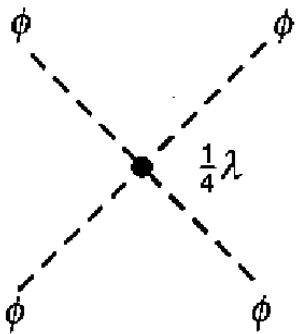
\includegraphics[width=0.2\linewidth]{higgs_boson/zelf_int_term_scal.png}
    \caption{Feynman diagram van de zelf interactie van het scalaire veld}%
    \label{fig:higgs_boson/zelf_int_term_scal}
\end{figure}

De potentiaal heeft enkel een minimum in $\phi=0$.

\begin{figure}[h]
    \centering
    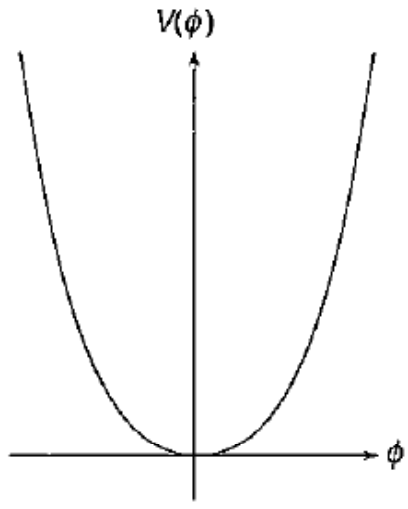
\includegraphics[width=0.2\linewidth]{higgs_boson/hoed_pot_1.png}
    \caption{De hoed potentiaal met $\mu^2>0$}%
    \label{fig:higgs_boson/hoed_pot_1}
\end{figure}

Nemen we nu $\mu^2<0$ krijgen we nu 2 minima in de potentiaal bij $\pm v$.

\begin{figure}[h]
    \centering
    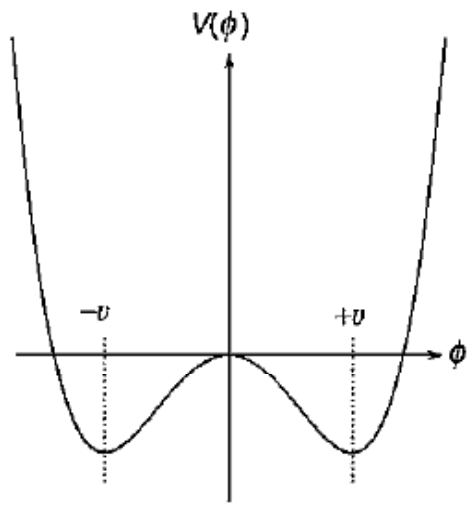
\includegraphics[width=0.2\linewidth]{higgs_boson/hoed_pot_2.png}
    \caption{De hoed potentiaal met $\mu^2<0$}%
    \label{fig:higgs_boson/hoed_pot_2}
\end{figure}

De tweede term is nu geen massaterm meer en hebben we een massaloos deeltje dat beweegt in een bepaalde potentiaal. De vacuum toestand wat de laagste toestand is ligt bij $\phi = \pm v = \pm \left| \sqrt{ \frac{-\mu^2}{\lambda}} \right|$. Dit is nu juist waar de symmetrie wordt gebroken. Nemen we nu de vacuum toestand bij $\phi = +v$ (hier maken we een verschil tussen $\pm v$ en breken we de symmetrie) is het mogelijk om $\phi$ te herschrijven.
\begin{equation}
    \begin{aligned}
        \label{eq:veld_symm_breking}
        \phi(x) &= v+\eta(x)
    \end{aligned}
\end{equation}
$\eta$ is hier de beschrijving van het deeltje in de put (hoeveel deze dus afwijkt van $v$). Vullen we dit in in vergelijking (\ref{eq:lagr_hoed_pot}) geeft het volgende
\begin{equation}
    \begin{aligned}
        \label{eq:lagr_hoed_pot_symm_breking}
        \mathcal{L} &= \frac{1}{2} (\partial_\mu \eta) (\partial^\mu \eta) - \frac{1}{2} \mu^2 (v+\eta)^2 - \frac{1}{4} \lambda (v+\eta)^4\\
                    &\downarrow \mu^2= v^2\lambda\\
        &= \frac{1}{2} (\partial_\mu \eta) (\partial^\mu \eta) - \lambda v^2\eta^2 - \lambda v \eta^3 - \frac{1}{4} \lambda \eta^4 + \frac{1}{4} \lambda v^4\\
    \end{aligned}
\end{equation}
Wat we nu kunnen zien is een massief scalair veld met $m_\eta = \sqrt{2\lambda v^2} = \sqrt{-2\mu^2}$ met 2 self interacties van het $\eta$ veld.

\begin{figure}[h]
    \centering
    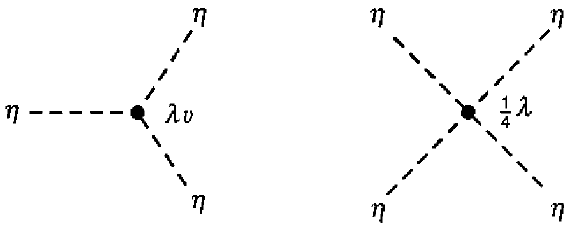
\includegraphics[width=0.4\linewidth]{higgs_boson/zelf_int_eta.png}
    \caption{Zelf interacties van het $\eta$ veld}%
    \label{fig:higgs_boson/zelf_int_eta}
\end{figure}

De laatste term in de Lagrangiaan is een constante en omdat de Lagrangiaan altijd in afgeleides voorkomt in bewegingsvergelijking is deze term niet relevant.

\subsection{Complexe scalaire velden}%
\label{sub:complexe_scalaire_velden}

Introduceren we de nu het complexe scalaire veld en de Lagrangiaan dat dat hierbij hoort.
\begin{equation}
    \begin{aligned}
        \label{eq:complex_scalair_veld}
        \phi &= \frac{1}{\sqrt{2}} (\phi_1 + i\phi_2)\\
        \mathcal{L} &= (\partial_\mu \phi)^*(\partial^\mu\phi) - \mu^2(\phi^*\phi) - \lambda(\phi^*\phi)^2
    \end{aligned}
\end{equation}
De hoed potentiaal zal in deze omstandigheden geroteerd worden rond de as loodrecht op het $\phi_1\phi_2$ vlak.

\begin{figure}[h]
    \centering
    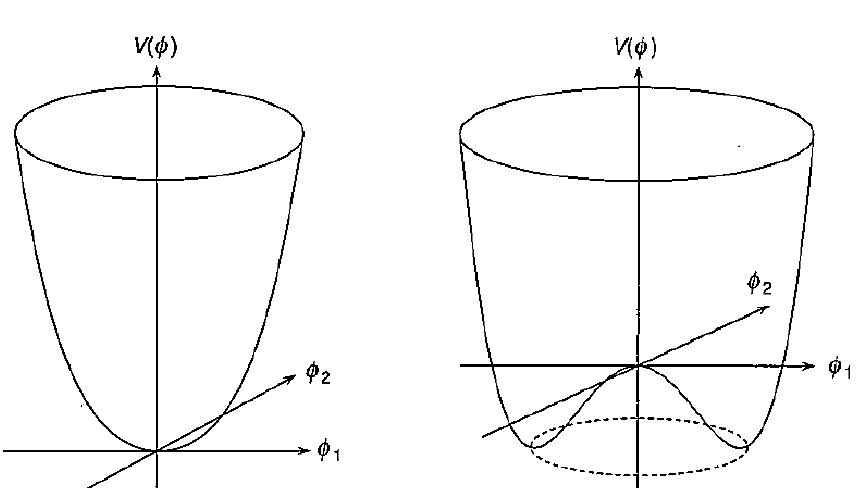
\includegraphics[width=0.6\linewidth]{higgs_boson/hoed_pot_comp.png}
    \caption{Complexe uitbreiding van de hoed potentiaal}%
    \label{fig:higgs_boson/hoed_pot_comp}
\end{figure}

Deze zal in dit geval invariant zijn onder de globale $U(1)$ transformatie $\phi \rightarrow e^{i\alpha}\phi$. Voor $\mu^2<0$ krijgen we nu een ring van minima bij
\begin{equation}
    \begin{aligned}
        \label{eq:complex_symm_breking}
        \phi_1^2+\phi_2^2 = -\frac{\mu^2}{\lambda} =v^2
    \end{aligned}
\end{equation}
We kiezen de vacuum toestand bij $(\phi_1, \phi_2) = (v,0)$ wat de globale $U(1)$ symmetrie spontaan zal breken. Expanderen we deze vacuum toestand en vullen we deze in de Lagrangiaan in dan krijgen we uiteindelijk:
\begin{equation}
    \begin{aligned}
        \label{eq:comple_scalair_veld_symm_breking}
        \phi_1(x) &= \eta(x) + v\\
        \phi_2(x) &= \xi(x)\\
        \mathcal{L} &= \frac{1}{2} (\partial_\nu \eta) (\partial^\mu \eta) + \frac{1}{2} (\partial_\nu \xi) (\partial^\mu \xi) - V(\eta, \xi)\\
        V(\eta, \xi) &= -\frac{1}{4} \lambda v^4 + \lambda v^2 \eta^2 + \lambda v \eta^3 + \frac{1}{4} \lambda \eta^4 + \frac{1}{4} \lambda \xi^4 + \lambda v \eta\xi^2 + \frac{1}{2} \lambda \eta^2\xi^2
    \end{aligned}
\end{equation}
Uit al deze termen kunnen we een aantal elementen waarnemen. Er is een scalair veld aanwezig met massa $m_\eta = \sqrt{2\lambda v^2}$ en een massaloos scalair veld $\xi$. Zoals te zien in de potentiaal kunnen deze 2 velden aan zelf interacties doen. Deze interacties komen overeen met de volgende diagrammen.

\begin{figure}[h]
    \centering
    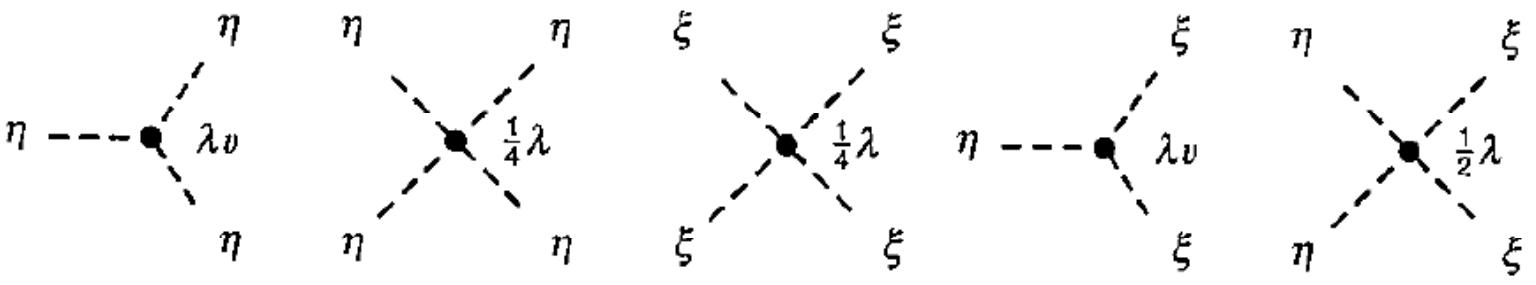
\includegraphics[width=0.8\linewidth]{higgs_boson/complex_scalair_veld_int.png}
    \caption{Zelf interactie diagrammen van complex scalair veld}%
    \label{fig:higgs_boson/complex_scalair_veld_int}
\end{figure}

Het massaloze deeltje komt overeen met de perturbatie van het deeltje langs de cirkel van minima. Om zich hierlangs te verplaatsen is er geen extra energie nodig en wil dit dus zeggen dat het massaloos is.

\subsubsection{Lokale ijk symmetrie}%
\label{ssub:lokale_ijk_symmetrie}

Gaan we nu over van de globale symmetrie naar de lokale $U(1)$ symmetrie moeten we de covariante afgeleide terug invoeren.
\begin{equation}
    \begin{aligned}
        \label{eq:complex_scalair_veld_lokaal}
        \phi(x) &\rightarrow \phi'(x) = e^{ig\chi(x)}\phi(x)\\
        \partial_\mu &\rightarrow D_\mu = \partial_\mu + igB_\mu\\
        B_\mu &\rightarrow B'_\mu = B_\mu - \partial_\mu \chi(x)
    \end{aligned}
\end{equation}
We voeren hier in essentie hetzelfde uit als sectie \ref{sub:lakale_u_1_gauge_invariantie} maar dan voor deeltjes met een andere potentiaal. Hierbij hebben we bij het vervangen van de afgeleide door een de covariante afgeleide terug een extra vector veld $B_\mu$ toegevoegd die de informatie zal dragen van de lokale fases. De Lagrangiaan wordt nu
\begin{equation}
    \begin{aligned}
        \label{eq:comp_scal_veld_lagr_lok_symm}
        \mathcal{L} = - \frac{1}{4} F^{\mu\nu}F^{\mu\nu} + (\partial_\mu \phi)^*(\partial^\mu \phi)-\mu^2\phi^2-\lambda\phi^4\\
        - igB\mu \phi^* (\partial^\mu \phi) + ig (\partial_\mu \phi)^* B^\mu \phi + g^2 B_\mu B^\mu \phi^* \phi
    \end{aligned}
\end{equation}
Hier krijgen we terug een aantal extra termen in de Lagrangiaan. We zien dat een massaloos ijkveld $F^{\mu\nu} = \partial^\mu B^\nu - \partial^\nu B^\mu$ is toegevoegd. De derde laatste toont ook dat dit massaloos ijkveld zal interageren met $\phi$. Werken we de symmetrie breking bij $\mu^2<0$ uit met $\phi(x)= \frac{1}{\sqrt{2}} (v + \eta(x) + i\xi(x))$ vinden we een nieuwe Lagrangiaan
\begin{equation}
    \begin{aligned}
        \label{eq:comp_scal_veld_lagr_lok_symm_breking}
        \mathcal{L} = {\color{red}\frac{1}{2} (\partial_\nu\eta)(\partial^\nu\eta) + \lambda v^2\eta^2} + {\color{blue}\frac{1}{2} (\partial_\nu\xi)(\partial^\nu\xi)} - {\color{green}V_{int}(\eta,\xi,B)}\\
        - {\color{orange}\frac{1}{4} F^{\mu\nu}F_{\mu\nu} + \frac{1}{2} g^2v^2B_\mu B^\mu} + {\color{purple}gvB_\mu(\partial^\mu \xi)}
    \end{aligned}
\end{equation}
In het rood vinden we de beschrijving van het scalair veld $\eta$ dat massief is geworden, in het blauw een massaloos scalaire veld $\xi$, in het groen de interacties tussen $\eta$, $\xi$ en $B$, in oranje het massieve B veld en ten laatste in het paars een directe koppeling van het $B$ veld met het $\xi$ veld. Maar wat is de laatste term nu? Deze klopt niet echt. Het is mogelijk om van deze term af te geraken door een specifieke ijk te kiezen en van daar alles te interpreteren. De ijk die we hier opleggen noemen we de unitaire ijk, $\chi(x) = -\xi(x)/gv$. De complexe term van de golffunctie wordt door deze ijk opgenomen door $v$ en geeft $\phi(x) = \frac{1}{\sqrt{2}} (v+\eta(x)) \equiv \frac{1}{\sqrt{2}} (v+h(x))$. Hierdoor komt $\xi(x)$ niet meer expliciet voor in de Lagrangiaan maar deze zal wel voorkomen in de transformaties $B_\mu (x) \rightarrow B'_\mu(x) - B_\mu(x) + \frac{1}{gv} \partial_\mu \xi(x)$.
\begin{equation}
    \begin{aligned}
        \label{eq:comp_scal_veld_lagr_unitaire_ijk}
        \mathcal{L} = \frac{1}{2} (\partial_\nu h)(\partial^\nu h) + \lambda v^2 h^2 + \frac{1}{2} (\partial_\nu\xi)(\partial^\nu\xi) - \frac{1}{4} F^{\mu\nu}F_{\mu\nu} + \frac{1}{2} g^2v^2B_\mu B^\mu\\
        + g^2vB_\mu B^\mu h + \frac{1}{2} g^2 B_\mu B^\mu h^2 - \lambda vh^3 - \frac{1}{4} \lambda h^4
    \end{aligned}
\end{equation}
Hierbij zijn de $\eta$ termen vervangen door Higgs termen. We hebben nog steeds het $B$ veld en de directe koppeling van $B$ en $\xi$ is verdwenen. De $\xi$ termen zijn als het ware opgeslokt door het $B$ veld. Zo bekomen we een Lagrangiaan die 2 massieve velden beschrijft met hun inderlinge interacties daarbij. De massa van deze velden zijn $m_B = gv$ en $m_h = \sqrt{2\lambda}v$.

\begin{figure}[h]
    \centering
    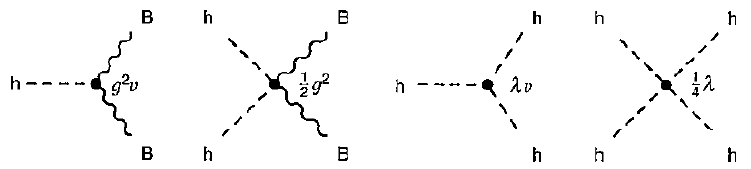
\includegraphics[width=0.8\linewidth]{higgs_boson/complex_scal_int_unitaire_ijk.png}
    \caption{Interactie diagrammen van de velden bij de unitaire ijk}%
    \label{fig:higgs_boson/complex_scal_int_unitaire_ijk}
\end{figure}

\subsection{Het standaard model scalair}%
\label{sub:het_standaard_model_scalair}

In het standaard model hebben we natuurlijk niet alleen lokale $U(1)$ ijk symmetrie maar hebben we eerder een lokale $SU(2)_L\times U(1)_Y$ ijk symmetrie. Deze zullen opbreken in 3 massieve velden $W^+$, $W^-$ en $Z$. Om dit te doen hebben we een scalair veld nodig met 4 vrijheidsgraden.
\begin{equation}
    \begin{aligned}
        \label{eq:sm_scalair_veld}
        \phi = 
        \begin{pmatrix}
            \phi^+\\
            \phi^-
        \end{pmatrix}
        = \frac{1}{\sqrt{2}} 
        \begin{pmatrix}
            \phi_1 + i\phi_2\\
            \phi_3 + i\phi_4
        \end{pmatrix}
    \end{aligned}
\end{equation}
Indien je dit helemaal zou uitwerken (zie Thomson) kan je de verschillende massa's voor de deeltjes: $m_W = \frac{1}{2} gv$, $m_A = 0$, $m_Z = \frac{1}{2} v\sqrt{g^2+g'^2}$ en $m_h = \sqrt{2\lambda}v$. Uit experimenten is het mogelijk om de massa's van deze deeltjes te bepalen en is het mogelijk om andere parameters te berekenen. Zo komt uit $m_W$ en $g$ dat het vacuum $v=246$GeV is. De reden hiervoor weten we niet. Uit $m_W$ en $m_Z$ kunnen we zoals we eerder al gezien hebben de Weinberg hoek $\theta_W$ bepalen. Het was uit de theorie nog niet mogelijk om de massa van het Higgs boson te bepalen omdat er nog een onbekende $\lambda$ was.

\begin{figure}[h]
    \centering
    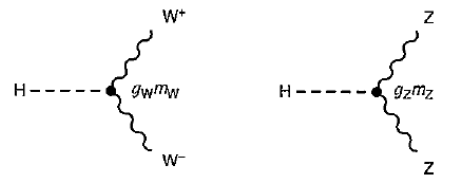
\includegraphics[width=0.6\linewidth]{higgs_boson/koppeling_higgs_wz_boson.png}
    \caption{Koppeling van $W$ en $Z$ aan het Higgs veld}%
    \label{fig:higgs_boson/koppeling_higgs_wz_boson}
\end{figure}

Voor de koppelingsconstante van deze deeltjes hebben we $g_W=g$, $g_Z= \frac{g}{\cos\theta_W}$ en zien we dat de koppeling van het $W$ en $Z$ boson aan het Higgs veld zullen afhangen van hun massa.\\
{\color{red} Het is hier niet de bedoeling om de Lagrangianen volledig te kunnen afleiden op het examen zoals hier is gedaan, het is veel belangrijker om de Lagrangianen te kunnen interpreteren en er de fysische betekenissen van kunnen geven.}

\subsection{Fermion massa's}%
\label{sub:fermion_massa_s}

\begin{figure}[h]
    \centering
    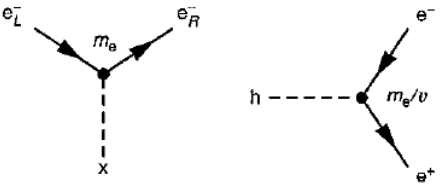
\includegraphics[width=0.6\linewidth]{higgs_boson/koppeling_higgs_e.png}
    \caption{Koppeling van fermionen aan het Higgs veld}%
    \label{fig:higgs_boson/koppeling_higgs_e}
\end{figure}

Zoals de $W$ en $Z$ bosonen krijgen de fermionen ook massa door te koppelen aan het Higgs boson. De koppelingsconstante tussen deze 2 is gegeven door $g_f = \sqrt{2} \frac{m_f}{v} = \frac{m_f}{\sqrt{2}m_W} g$. Deze koppelingen zitten echter niet verwerkt in het Standaard Model. Deze moeten gemeten worden:
\begin{equation}
    \begin{aligned}
        \label{eq:kc_h_fermionen}
        g_t &= 0.997 \pm 0.006\\
        g_e &\approx 3\cdot 10^{-6}\\
        g_\nu &\leq 10^{-12}
    \end{aligned}
\end{equation}
Je kan ook inzien dat bij het interageren van fermionen met het Higgs veld (eerste diagram in figuur \ref{fig:higgs_boson/koppeling_higgs_e}) gaat via links en rechts chirale deeltjes wat de koppeling tussen neutrinos en het Higgs veld onmogelijk zal maken.\\
Vroeger was de vraag waarom de top quark zo zwaar was. Dit is eigenlijk de normaal en moeten we ons af vragen waarom de andere fermionen zo licht koppelen aan het Higgs veld.

\subsection{Higgs verval}%
\label{sub:higgs_verval}

\begin{figure}[h]
    \centering
    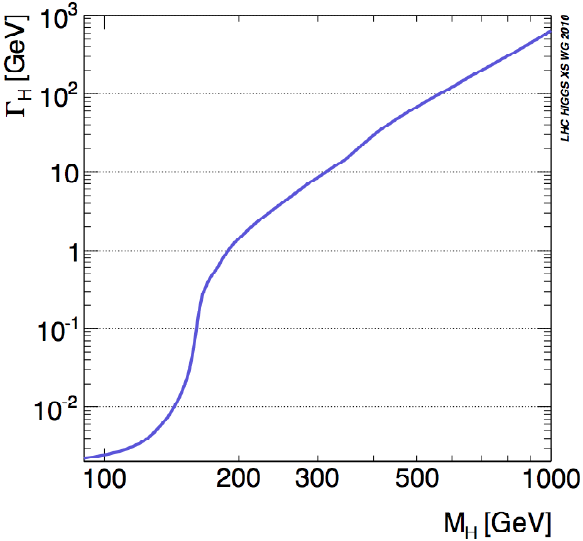
\includegraphics[width=0.5\linewidth]{higgs_boson/verval_breedte_higgs.png}
    \caption{Verval breedte van het Higgs boson in functie van zijn massa}%
    \label{fig:higgs_boson/verval_breedte_higgs}
\end{figure}

Nu we een model hebben voor het Higgs boson is het natuurlijk ook belangrijk om na te gaan of deze ook echt klopt. Het nagaan van de theorie doen we natuurlijk aan de hand van experimenten waar we dat Higgs boson moeten kunnen waarnemen. Het Higgs boson heeft meerdere verval kanalen met elk hun typische karakteristieken.
\begin{itemize}
    \item $H\rightarrow f\overline f$: De vervalbreedte van deze fermion vervalkanalen hangen door de massa afhankelijkheid van de koppelingsconstante ook af van de massa's van de interagerende deeltjes, $\Gamma(H\rightarrow f\overline f) \propto m_f^2m_H$. Behalve als $m_H > 2m_t$ (wat heel onwaarschijnlijk is vanwege de grote massa van het top quark) is zal het sterkste fermionisch verval kanaal gegeven worden door $b\overline b$.
    \item $H\rightarrow WW$: Het Higgs boson koppelt ook sterk aan de $W$ bosonen met $\Gamma(H\rightarrow WW)\propto m_H^3$ als $m_H \gg 2m_W$. Daarentegen als $m_H < 2m_W$ moet minstens 1 $W$ off-shell zijn wat onderdrukt zal worden.
    \item $H\rightarrow ZZ$: Als hier terug $m_H \gg 2m_Z$ krijgen we $\Gamma(H\rightarrow ZZ)\propto \Gamma(H\rightarrow WW)/2$.
    \item $H\rightarrow \gamma\gamma$ en $H \rightarrow gg$: Niet op boom level wat we later bekijken.
\end{itemize}
De totale verval breedte van het Higgs boson wordt gegeven door $\Gamma_{tot} = \sum_X \Gamma(H\rightarrow XX)$ en kan geplot worden in functie van de massa van het Higgs boson. Onder de $150$GeV is $\Gamma_H$ klein omdat er niet veel mogelijke verval kanalen zijn. Vanaf je aan de $180$GeV komt is het mogelijk om 2 $W$ bosonen aan te maken en vergroot $\Gamma_H$  significant. Als je kijkt bij $m_H=1000$GeV is zijn breedte even groot en zou het experimenteel onmogelijk zijn om deze waar te nemen. In figuur \ref{fig:higgs_boson/verval_higgs} worden de waarschijnlijkheden gegeven om het Higgs te laten vervallen naar een specifiek kanaal. Hier wordt bevestigd dat bij lage energie $b\overline b$ overheerst en vanaf $\pm 150$GeV zal $WW$ verval overnemen. Een interessante opmerking is dat de waarschijnlijkheid van het $Z$ boson een dip zal ondervinden bij de $W$ resonantie.

\begin{figure}[h]
    \centering
    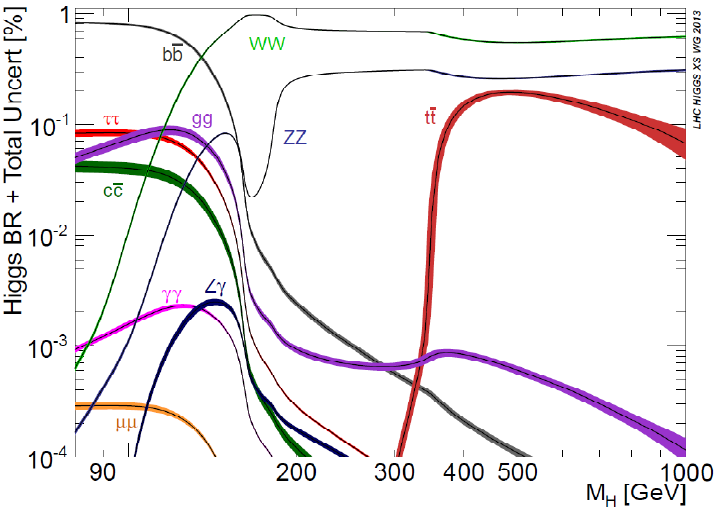
\includegraphics[width=0.6\linewidth]{higgs_boson/verval_higgs.png}
    \caption{Waarschijnlijkheid van de verschillende Higgs verval kanalen}%
    \label{fig:higgs_boson/verval_higgs}
\end{figure}

We zien ook nog dat $gg$ en $\gamma\gamma$ een bijdrage zal geven tot de vervalbreedte wat niet zou mogen omdat deze niet binden aan het Higgs boson. In het LEP was het maar mogelijk om metingen te doen tot $130$GeV. In tabel \ref{tab:h_verval_125_gev} kan je de waarschijnlijkheden vinden waarin het Higgs zou vervallen als $m_H=125$GeV is.

\begin{table}[h]
    \centering
    \caption{Verval waarschijnlijkheid van Higgs bij $m_h=125$GeV}
    \label{tab:h_verval_125_gev}
    \begin{tabular}{cc}
        Verval modes & vertakking \\
        $H\rightarrow b\overline b$ & $57.8\%$ \\
        $H\rightarrow WW^*$ & $21.6\%$ \\
        $H\rightarrow \tau^+\tau^-$ & $6.4\%$ \\
        $H\rightarrow gg$ & $8.6\%$ \\
        $H\rightarrow c\overline c$ & $2.9\%$ \\
        $H\rightarrow zz^*$ & $2.7\%$ \\
        $H\rightarrow \gamma\gamma$ & $0.2\%$ \\
    \end{tabular}
\end{table}

\subsubsection{Higgs verval naar $\gamma\gamma$ en $gg$}%
\label{ssub:higgs_verval_naar_gammagamma_en_gg_}

Kijken we nu hoe het Higgs boson toch kan vervallen naar de massaloze bosonen die niet koppelen met het Higgs boson. De feynman diagrammen voor deze vervallen worden gegeven in figuur \ref{fig:higgs_boson/h_naar_foton_gluon}.

\begin{figure}[h]
    \centering
    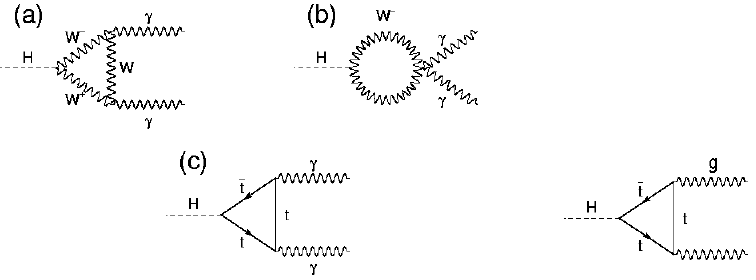
\includegraphics[width=0.8\linewidth]{higgs_boson/h_naar_foton_gluon.png}
    \caption{Diagrammen van het Higgs verval naar massaloze bosonen}%
    \label{fig:higgs_boson/h_naar_foton_gluon}
\end{figure}

Alle informatie van alle deeltjes zal beschreven worden in de lussen. Indien er nog een zwaarder quark zou bestaan dan de top quark zou deze ook een bijdrage leveren. Deze diagrammen zullen nog steeds maar een kleine bijdrage aan de totale vervalbreedte. Dit wil zeggen dat er maar een kleine hoeveelheid fotonen worden aangemaakt. De reden waarom we hier zo geïnteresseerd in zijn is omdat fotonen zo makkelijk te detecteren zijn in tegenstelling tot de bottom quarks die zo overvloedig aanwezig zijn. Over het waarnemen van de Higgs bosonen zullen we later verder op in gaan.

\subsection{Higgs productie}%
\label{sub:higgs_productie}

Het produceren van Higgs bosonen is een hele taak op zichzelf. In de $e^+e^-$ colliders is het in essentie mogelijk dat het elektron en positron annihileren in elkaar ($e^+e^-\rightarrow H$) maar dit is zo goed als onmogelijk vanwege de massa van het elektron. Wat wel een mogelijkheid zal zijn om Higgs bosonen aan te maken noemen we ``Higgs-strahlung''.

\begin{figure}[h]
    \centering
    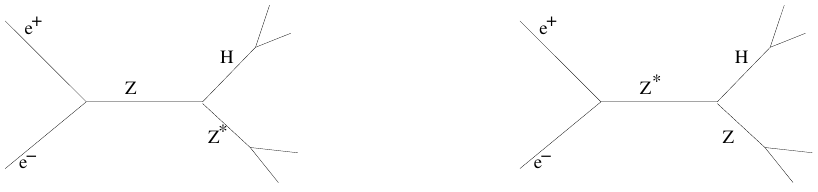
\includegraphics[width=0.6\linewidth]{higgs_boson/Higgs_strahlung.png}
    \caption{Diagrammen van Higgs-strahlung}%
    \label{fig:higgs_boson/Higgs_strahlung}
\end{figure}

Deze Higgs-strahlung kan ook gedaan worden met quarks en kan naast het gebruiken van een $Z$ boson ook een $W$ boson gebruikt worden. Dit wordt ook wel geassocieerde productie van het Higgs bij een vector boson genoemd. Een andere mogelijkheid om Higgs bosonen te maken is de vector-boson fusie. Dit zal vooral voorkomen bij quarks maar is technisch gezien ook mogelijk bij het botsen van elektronen.

\begin{figure}[h]
    \centering
    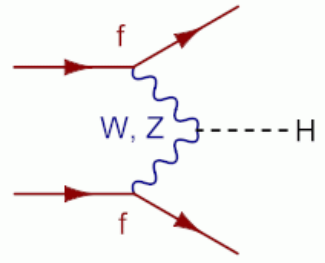
\includegraphics[width=0.5\linewidth]{higgs_boson/vec_bos_fusie.png}
    \caption{Feynman diagram voor vector-boson fusie}%
    \label{fig:higgs_boson/vec_bos_fusie}
\end{figure}

Hier stralen 2 verschillende quarks een $W$ of $Z$ uit om te combineren tot een Higgs boson. Nog een andere mogelijkheid die enkel mogelijk is bij hadron colliders is de $t\overline t$ fusie. Hier vervallen 2 gluonen tot $t\overline t$ paren waar de centrale $t\overline t$ zullen annihileren tot een Higgs boson.

\begin{figure}[h]
    \centering
    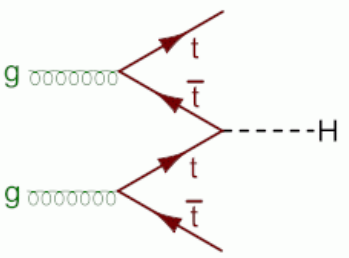
\includegraphics[width=0.5\linewidth]{higgs_boson/tt_fusie.png}
    \caption{Feynman diagram voor $t\overline t$ fusie}%
    \label{fig:higgs_boson/tt_fusie}
\end{figure}

Dit is een heel handige vorm van Higgs productie omdat de top quarks en Higgs boson makkelijk te onderscheiden zijn. Ten laatste hebben we nog een productie die enkel mogelijk is in hadron colliders. De gluon-gluon fusie waar enkel een Higgs boson zal aangemaakt worden.

\begin{figure}[h]
    \centering
    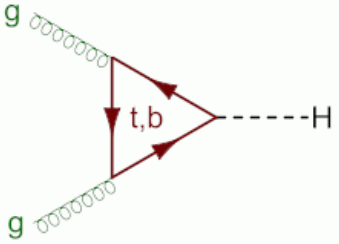
\includegraphics[width=0.5\linewidth]{higgs_boson/gluon_gluon_fusie.png}
    \caption{Feynman diagram voor gluon gluon fusie}%
    \label{fig:higgs_boson/gluon_gluon_fusie}
\end{figure}

Kijken we nu eens naar de werkzame doorsnedes van al deze processen in een hadron collider indien we de massa van het Higgs boson nog niet weten. In figuur \ref{fig:higgs_boson/h_prod_lhc} worden de werkzame doorsnedes van alle producties uitgezet in functie van de massa van het Higgs boson.

\begin{figure}[h]
    \centering
    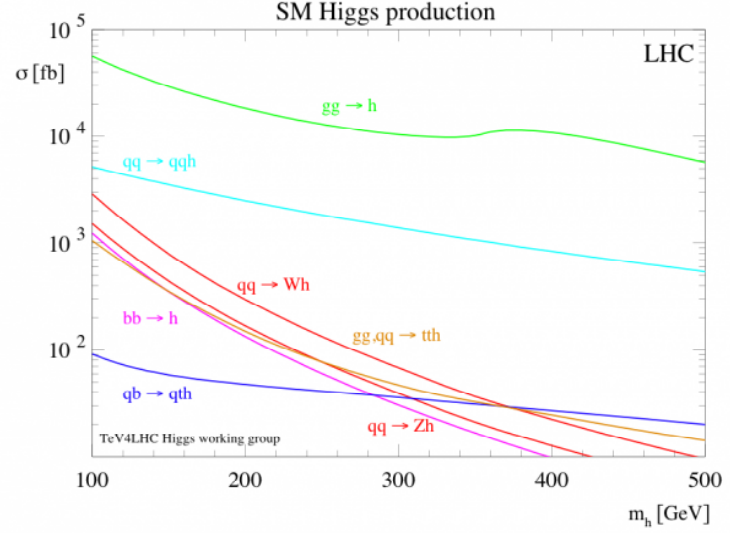
\includegraphics[width=0.6\linewidth]{higgs_boson/h_prod_lhc.png}
    \caption{Werkzame doorsnedes van Higgs productie in functie van zijn massa}%
    \label{fig:higgs_boson/h_prod_lhc}
\end{figure}

Belangrijk om op te merken hier is dat de werkzame doorsnedes hier de eenheid femtobarn gebruiken wat heel klein is. Het is duidelijk dat de gluon gluon fusie het belangrijkste kanaal zal zijn. Op de 2de plaats vinden we de vector-boson fusie.

\subsection{De zoek voor het Higgs boson}%
\label{sub:de_zoek_voor_het_higgs_boson}

De initiële zoektocht naar het Higgs boson is begonnen in het LEP. Dit is dus de geassocieerde productie $e^{+} e^{-} \rightarrow Z+H$. Eens het Higgs aangemaakt is zal het voornamelijk vervallen naar $b$ quarks ($H \rightarrow b \bar{b}$) en het $Z$ boson zal vervallen in 3 mogelijke combinaties $Z \rightarrow l^{+} l^{-}, \nu \bar{\nu}, q \bar{q}$. Het probleem bij deze opstelling is dat er een sterke achtergrond zal zijn voor $e^{+} e^{-} \rightarrow Z+Z^{*}$ waar bij het virtueel boson vervalt naar $Z^{*} \rightarrow b \bar{b}$. De maximale hoeveelheid energie dat aangemaakt kan worden in het LEP is $\sqrt{s} = 209$GeV. Nemen we hiervan dan nog eens de massa van het $Z$ boson af kunnen we maar zoeken naar een Higgs boson met een massa kleiner dan $m_{H}<\sqrt{s}-m_{Z}=118$GeV. In de praktijk valt nog een kleine hoeveelheid weg door waarnemings thresholds en zou de massa van het Higgs kleiner moeten zijn dan $114$GeV.\\
Schakelen we over naar het Tevatron en LHC waar we veel hogere energieën kunnen berijken. Kijken we eerst naar het Tevatron waar $p\bar{p}$ of in essentie een quark en antiquark zullen botsen met elkaar. Het grote nadeel voor de hadron colliders is natuurlijk dat deze een grote hoeveelheid achtergrond creëren. Om deze achtergrond een beetje te proberen omzeilen kijken we het liefst naar de geassocieerde productie van Higgs bosonen. Dit omdat we hier een $t\bar{t}$ of een $W$ of een $Z$ wordt aangemaakt die we dan kunnen gebruiken als tags. De verschillende vervalmodes zijn:
\begin{itemize}
    \item $b\bar{b}$: deze is geprefereerd maar is moeilijk om waar te nemen in hadron colliders omdat er duizenden mogelijkheden zijn om deze aan te maken.
    \item $\tau^{+} \tau^{-}$: iets minder moeilijk maar nog steeds moeilijk omdat je het $\tau$ zelf niet ziet vanwege zijn korte levensduur.
    \item $W^+W^-$: dit is een heel mooie vervalmode met $l_{1} \nu l_{2} \nu$ en krijg je een elektron positron paar met tegengestelde impulsen. Jammer genoeg is dit moeilijk te reconstrueren vanwege de 2 onbekende impulsen van deneutrinos.
    \item $Z Z^{*} \rightarrow l_{1}^{+} l_{2}^{-} l_{3}^{+} l_{4}^{-}$: Dit is het gouden kanaal omdat deze heel makkelijk te reconstrueren zijn tot het reële en virtuele $Z$ boson.
    \item $\gamma\gamma$: ondanks heel onwaarschijnlijk te zijn is dit toch interessant vanwege de makkelijke detectie.
\end{itemize}
Om dit alles goed uit te voeren is het nodig een een zoek criterium in te voeren. Voor een gegeven $m_H$ moeten de volgende stappen ondernomen worden:
\begin{enumerate}
    \item Criterium selecteren: Kijk ik naar 2$\gamma$'s of naar 4 leptonen uit $ZZ^*$?
    \item Tel alle mogelijke kandidaten voor dit criterium bij bepaalde $m_H$.
    \item Vergelijk deze tot de verwachte Standaard Model achtergrond. Dit zijn dus alle mogelijke processen om bijvoorbeeld $\gamma$'s te creëren.
    \item Gebruik de statistieken om te probabiliteit te berekenen dat dit een Higgs deeltje is.
    \item Zo hebben we het aantal Higgs deeltjes waar we $95\%$ zeker van zijn dat ze een Higgs deeltje zijn: $N_{95}$.
    \item Bereken de cross sectie hiervan: $\sigma_{95}=N_{95} /(\epsilon \cdot \mathcal{L})$.
    \item Vergelijk dit met de theorie: $R_{95}=\frac{\sigma_{95}}{\sigma_{S M}}$. Hierbij is $\sigma_{S M}$ de werkzame doorsnede die we verwachten uit de theorie.
\end{enumerate}
Als $R<1$ dan zijn we met $95\%$ kans zeker dat de gemeten werkzame doorsnede kleiner is dan de theorie en hebben we $95\%$ kans dat er geen Higgs zal zijn bij deze massa.\\
Heel belangrijk bij deze experimenten is om een grote hoeveelheid evenementen te bekijken zodat de werkzame doorsnede van de $95\%$ kan uitmiddelen tegenover de achtergrond. Indien dit niet gedaan wordt is de waarde van $R$ zo groot dat deze irrelevant zijn.\\
Bekijken we eerst de resultaten die gevonden zijn in het Tevatron. Indien de massa van het Higgs boson tussen $100-120$GeV uit $H \rightarrow b \bar{b}$ en tussen $139-184$GeV uit $H \rightarrow W W$ zou liggen zou deze met het Tevatron zeker waargenomen worden. In figuur \ref{fig:higgs_boson/zoektoacht_h_tevatron} zou die curve $R$ onder 1 moeten komen liggen als deze er niet zou liggen. Indien deze daar wel zou liggen zou in de experimenten $R$ boven 1 moeten blijven liggen en ontstaat er een exces tussen de vooraf verwachte (berekende) stippellijn en de experimentele waardes. In de werkelijkheid heeft het Tevatron het Higgs boson enkel kunnen uitsluiten voor massa's tussen $100-103$GeV en $147-180$GeV die weergegeven worden met de groene zones. De reden waarom het niet kon uitgesloten worden voor de energieën daartussen is door de overgang van het dominerende verval kanaal van het Higgs en de achtergrond proportioneel veel groter zal zijn in deze zones (zie figuur \ref{fig:higgs_boson/verval_higgs}).

\begin{figure}[h]
    \centering
    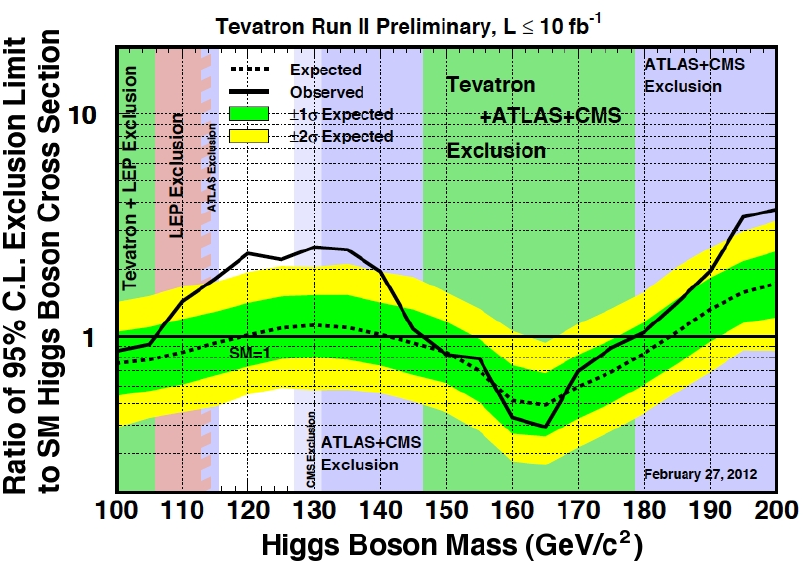
\includegraphics[width=0.6\linewidth]{higgs_boson/zoektoacht_h_tevatron.png}
    \caption{$R$ in functie van de Higgs massa in het Tevatron experiment}%
    \label{fig:higgs_boson/zoektoacht_h_tevatron}
\end{figure}

Op de verwachte waarde (stippellijn) hebben we natuurlijk een bepaalde zekerheid dat ze correct zijn. De groene en gele zones rond de verwachte lijnen geven de $1\sigma$ en $2\sigma$ waarschijnlijkheid weer. Indien er weldegelijk een Higgs boson aanwezig zou zijn moet er een exces zijn tussen de experimentele waardes en de voorspelde waarden. Dit omdat de voorspelde waarden voor $R$ bij het meten van meer experimenten enkel kan dalen maar de experimentele $R$ naar 1 zal moeten gaan omdat de experimentele werkzame doorsnede naar de werkzame doorsnede van het Standaard Model zal convergeren. Het Tevatron zegt dus dat er iets zal zitten rond die $124$GeV waar we het Higgs nu juist verwachten. Dit exces van $\pm 2.5\sigma$ is deze niet groot genoeg om het Higgs boson als ontdekt te beschouwen. Eén van de grote redenen hiervoor is de breedte van het exces. Dit is zuiver uit experimentele limitaties. We hebben dus detectoren nodig die een betere resolutie hebben en maar data kunnen generen.\\
Hier komt het LHC dan in het beeld met een hogere $\sqrt{s}$ waardoor het makkelijker is om Higgs bosonen aan te maken en een hogere $\mathcal{L}$ waardoor zo goed als even veel evenementen kunnen uitgevoerd worden in 1 dag als er evenementen in een jaar kunnen aangemaakt worden in het Tevatron. Na een jaar experimentele data te verzamelen in het LHC krijgen we de resultaten weergegeven in figuur \ref{fig:higgs_boson/zoektocht_naar_h}.

\begin{figure}[h]
    \centering
    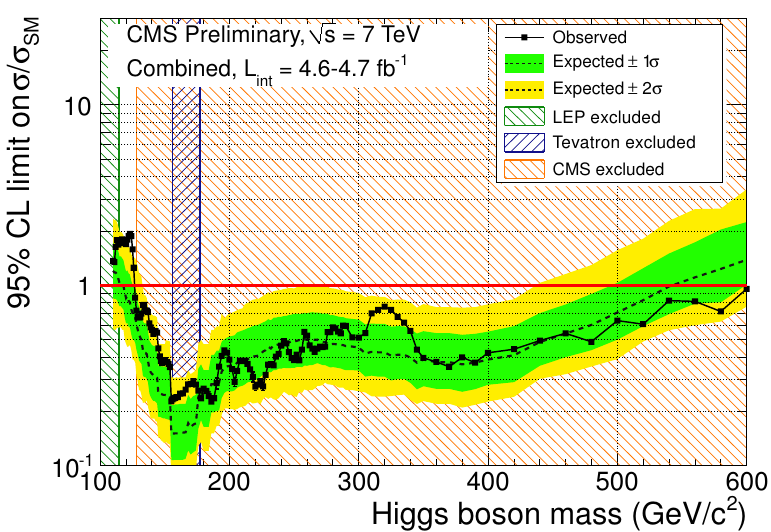
\includegraphics[width=0.6\linewidth]{higgs_boson/zoektocht_naar_h.png}
    \caption{$R$ in functie van de Higgs massa}%
    \label{fig:higgs_boson/zoektocht_naar_h}
\end{figure}

Zoals we hebben gezien in het Tevatron is er in het gebied rond $125$GeV terug een exces. Alles boven de $130$Gev kan nu uitgesloten worden. Blazen we dit exces nu even op in figuur \ref{fig:higgs_boson/zoektocht_h_zoom} zien we dat het Higgs boson zou liggen bij de $124$GeV wat niet echt een verrassing was.

\begin{figure}[h]
    \centering
    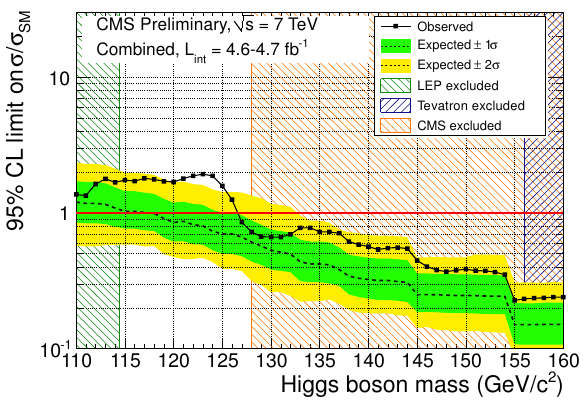
\includegraphics[width=0.6\linewidth]{higgs_boson/zoektocht_h_zoom.png}
    \caption{Zoom van figuur \ref{fig:higgs_boson/zoektocht_naar_h} rond het exces}%
    \label{fig:higgs_boson/zoektocht_h_zoom}
\end{figure}

Terug een jaar later wordt onderzocht hoe de werkzame doorsnede zich gedraagt in functie van de massa. Hier worden in figuur \ref{fig:higgs_boson/sigma_h_zoektocht} in de rode stippelijn de verwachte werkzame doorsnedes gegeven met hun waarschijnlijkheid en in de volle rode lijn de experimentele werkzame doorsnedes gegeven.

\begin{figure}[h]
    \centering
    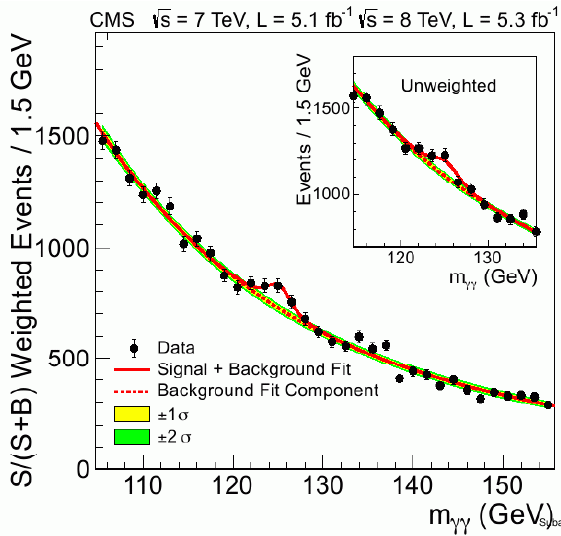
\includegraphics[width=0.4\linewidth]{higgs_boson/sigma_h_zoektocht.png}
    \caption{Werkzame doorsnedes van de voorspellingen en het experiment in functie van $m_H$}%
    \label{fig:higgs_boson/sigma_h_zoektocht}
\end{figure}

Omdat we weten uit het LEP en Tevatron dat het Higgs in bepaalde gebieden niet kon zitten konden we een bleit (geen idee hoe ik dit moet schrijven) analyse gedaan om er zeker van te zijn dat we geen bias hebben in de onderzoeksmethode. De gegevens werden initieel enkel geanalyseerd in de zones waar we wisten dat het Higgs niet zat om na te gaan dat alles klopt. Nu we weten dat onze analyse klopt kunnen we met dezelfde analyse kijken naar het gebied waar het Higgs wel verwachten. Uit deze analyse zien we dan uiteindelijk met een groot genoeg exces dat het Higgs bij $m_H=124$GeV ligt. {\color{blue} Intermezzo: Het verschil tussen de weighted en unweigted resultaten is de efficientie of het $\gamma\gamma$ dat gemeten is echt wel een $\gamma\gamma$ was en geen elektron of positron.}

\begin{figure}[h]
    \centering
    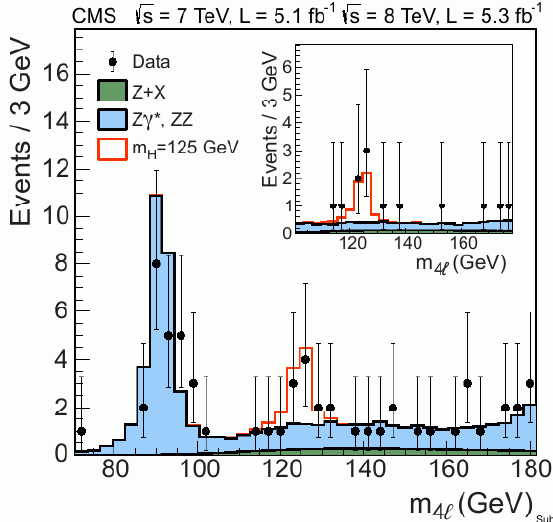
\includegraphics[width=0.5\linewidth]{higgs_boson/sigma_h_z_verval.png}
    \caption{Ontdekking van het $H$ aan de hand van zijn $ZZ^*$ verval}%
    \label{fig:higgs_boson/sigma_h_z_verval}
\end{figure}

Deze resultaten waren tot nu toe altijd voor het $\gamma\gamma$ verval. Dezelfde resultaten zijn gevonden voor het Higgs verval naar 2 $Z$ bosonen (figuur \ref{fig:higgs_boson/sigma_h_z_verval}).\\
Dit kan voor alle andere verval kanalen ook gedaan worden en als we deze samen plaatsen krijgen we mooi 1 piek.

\begin{figure}[h]
    \centering
    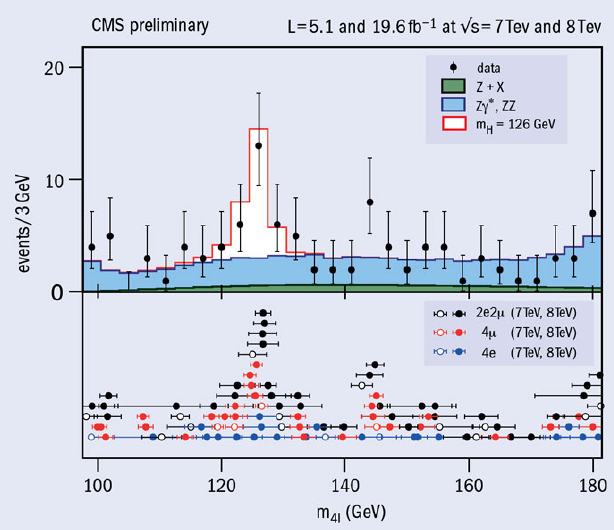
\includegraphics[width=0.5\linewidth]{higgs_boson/sigma_h_alles.png}
    \caption{Ontdekking van het $H$ voor alle verval kanalen samen}%
    \label{fig:higgs_boson/sigma_h_alles}
\end{figure}

\subsection{Eigenschappen van het nieuwe deeltje}%
\label{sub:eigenschappen_van_het_nieuwe_deeltje}

De massa van het Higgs boson is $m_H=125.8\pm0.4\text{(stat)}\pm 0.4\text{(syst)}$GeV en de koppeling met versschillende deeltjes kan je vinden in figuur \ref{fig:higgs_boson/h_koppeling}.

\begin{figure}[h]
    \centering
    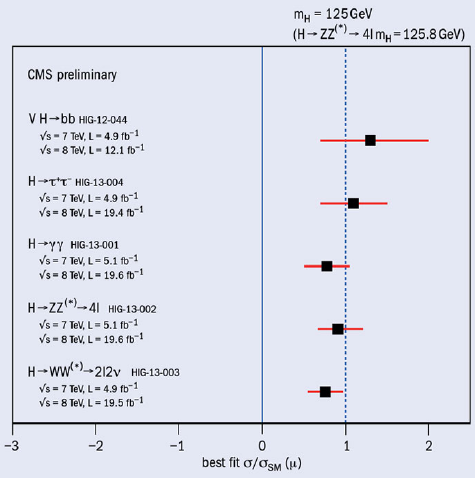
\includegraphics[width=0.5\linewidth]{higgs_boson/h_koppeling.png}
    \caption{Koppeling van H aanverschillende deeltjes}%
    \label{fig:higgs_boson/h_koppeling}
\end{figure}

Zetten we deze koppeling nu uit in functie van de koppeling aan fermionen en aan vector bosonen. Het Higgs boson is gemaakt om te koppelen aan de vector bosonen maar is niet verplicht om te koppelen aan de fermionen m.a.w. een fermiofoob deeltje. Indien dit zo zou zijn was dat zalig geweest en moesten we een nieuwe vorm vinden om massa te geven aan de fermionen. Jammer genoeg is dit niet het geval en zal deze wel koppelen met fermionen en deze massa geven aan hun.

\begin{figure}[h]
    \centering
    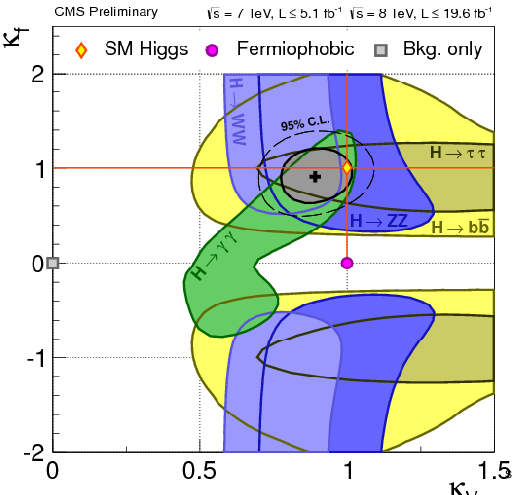
\includegraphics[width=0.5\linewidth]{higgs_boson/k_koppeling_vec_ferm.png}
    \caption{Koppeling van H aan vector bosonen en fermionen}%
    \label{fig:higgs_boson/k_koppeling_vec_ferm}
\end{figure}

Uit de theorie hebben we gezien dat de koppelingsconstante tussen H en andere deeltjes lineair af moeten hangen van hun massa. In figuur \ref{fig:higgs_boson/h_koppeling_massa} wordt deze gemeten relatie mooi weergegeven.

\begin{figure}[h]
    \centering
    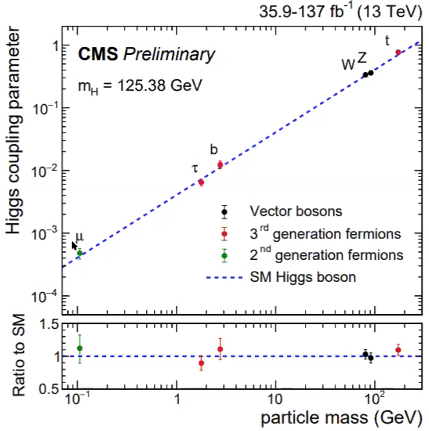
\includegraphics[width=0.4\linewidth]{higgs_boson/h_koppeling_massa.png}
    \caption{Relatie tussen de koppeling van H en de massa van het koppelende deeltje}%
    \label{fig:higgs_boson/h_koppeling_massa}
\end{figure}

Het Higgs deeltje doet dus exact wat we verwachten wat leuk is maar toch spijtig omdat we geen hints krijgen voor enige verdere fysica.\\
Uit het verval van he Higgs naar 2 fotonen weten we direct het een boson is. Om na te gaan dat het een scalair boson is met spin 0 moet er analyse gedaan worden van de hoek distributies.

\begin{figure}[h]
    \centering
    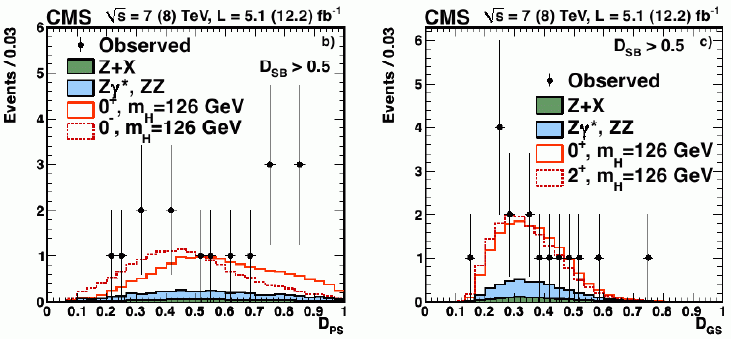
\includegraphics[width=0.5\linewidth]{higgs_boson/h_hoek_dist.png}
    \caption{Hoek distributies van het Higgs boson}%
    \label{fig:higgs_boson/h_hoek_dist}
\end{figure}

Uit verdere analyse kan ingezien worden dat dit een pseudo scalair boson moet zijn ($0+$ in figuur, pseudo deeltjes hebben een positieve pariteit)

\begin{figure}[h]
    \centering
    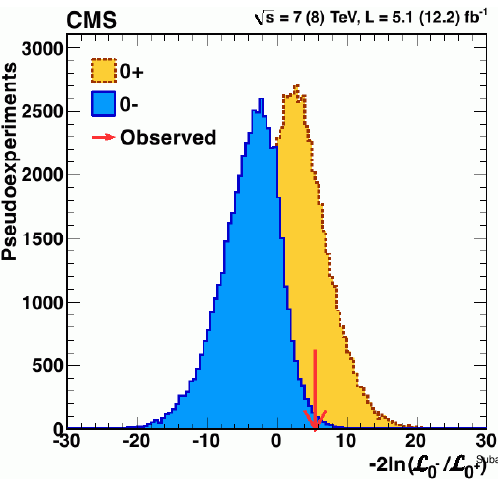
\includegraphics[width=0.5\linewidth]{higgs_boson/h_vec_boson.png}
    \caption{Nagaan of $H$ een scalair of pseudoscalair boson is}%
    \label{fig:higgs_boson/h_vec_boson}
\end{figure}

\end{document}
